\chapter{Discrete Random Variables}

\section{Random Variables}

\begin{definition}
    A \vocab{random variable} is a variable whose possible values are numerical outcomes of a random experiment.
\end{definition}

Random variables are typically denoted by capital letters such as $X$ or $Y$.

There are two types of random variables: discrete and continuous.

\begin{definition}
    A \vocab{discrete random variable} is a random variable that assumes countable values $x_1$, $x_2$, $\dots$, $x_n$ (can be infinite).
\end{definition}

Examples of discrete random variables include the number that shows on the toss of a fair die ($X = 1, 2, \dots, 6$), and the number of times a fair die is thrown until a `6' is obtained ($Y = 1, 2, \dots,$ to infinity).

In this chapter, we will only discuss discrete random variables. We will deal more with continuous random variables in \SS\ref{chap:Continuous-Random-Variables}.

\section{Properties}

\subsection{Probability Distribution}

Since the values of a random variable are determined by chance, there is a distribution associated with them. We call this a probability distribution.

\begin{definition}
    A \vocab{probability distribution} describes all possible values of the random variable and their corresponding probabilities. It assigns a probability value to each possible outcome in the sample space.
\end{definition}

A probability distribution of a discrete random variable can be given in the form of a table, a graph or a mathematical formula.

Note that the particular values of a random variable are denoted by lower-case letters. For instance, the particular values of a random variable $X$ are denoted by $x$.

\begin{example}[Probability Distribution]
    A single fair 6-sided die is thrown. Let $X$ be the random variable representing the number of dots showing on the die. Note that the possible values of $X$ are $x = 1, 2, 3, 4, 5, 6$.

    The probability distribution associated with $X$ can be given in table form:
    \begin{center}
        \begin{tabular}{|r|c|c|c|c|c|c|}
            \hline
            $x$ & 1 & 2 & 3 & 4 & 5 & 6 \\ \hline
            $\P{X = x}$ & $1/6$ & $1/6$ & $1/6$ & $1/6$ & $1/6$ & $1/6$ \\ \hline
        \end{tabular}
    \end{center}
    or expressed as a formula: \[\P{X = x} = \frac16, \quad x \in \bc{1, 2, 3, 4, 5, 6},\] or expressed as a graph:
    \begin{center}\tikzsetnextfilename{415}
        \begin{tikzpicture}
            \draw[->] (0, -1) -- (0, 2) node[anchor=east] {$\P{X = x}$};
            \draw[->] (-1, 0) -- (7, 0) node[anchor=west] {$x$};
            \draw (0.1, 1) -- (-0.1, 1) node[anchor=east] {$1/6$};

            \draw[thick] (1, 1) -- (1, 0) node[anchor=north] {1};
            \draw[thick] (2, 1) -- (2, 0) node[anchor=north] {2};
            \draw[thick] (3, 1) -- (3, 0) node[anchor=north] {3};
            \draw[thick] (4, 1) -- (4, 0) node[anchor=north] {4};
            \draw[thick] (5, 1) -- (5, 0) node[anchor=north] {5};
            \draw[thick] (6, 1) -- (6, 0) node[anchor=north] {6};

            \fill (1, 1) circle[radius=2.5pt];
            \fill (2, 1) circle[radius=2.5pt];
            \fill (3, 1) circle[radius=2.5pt];
            \fill (4, 1) circle[radius=2.5pt];
            \fill (5, 1) circle[radius=2.5pt];
            \fill (6, 1) circle[radius=2.5pt];
        \end{tikzpicture}
    \end{center}
\end{example}

From the above example, the discrete random variable $X$ takes on only countable values, and that if we sum all probabilities, we get a total of 1. In fact, these are conditions that all discrete random variables must satisfy.

\begin{condition}[Discrete Random Variable]
    For $X$ to be a discrete random variable,
    \begin{itemize}
        \item $X$ can take only countable values (finite or infinitely many), and
        \item $X$ has a probability distribution such that $0 \leq \P{X = x} \leq 1$ for all $x$ and \[\sum_{x} \P{X = x} = 1.\]
    \end{itemize}
\end{condition}

\subsection{Expectation}\label{ssec:DRV-Exp}

Recall that in descriptive statistics, the mean of a sample can be calculated as \[\text{Mean} = \frac{\sum xf}{n},\] where $x$ is a data value and $f$ is its frequency. In the case of a discrete random variable $X$, we can think of $x$ as a particular value of $X$, and $f/n$ as the probability that $x$ occurs (i.e. how ``frequently'' $x$ occurs). Thus, \[\text{Mean} = \sum_{x} x \P{X = x}.\] We call this ``mean'' the expectation of $X$.

\begin{definition}
    The \vocab{expectation}, or \vocab{expected value}, of $X$, denoted as $\E{X}$ or $\m$, is given by \[\E{X} = \sum_{x} x \P{X = x}.\]
\end{definition}

\begin{example}[Expectation]
    A single fair 6-sided die is thrown. Let $X$ be the random variable representing the number of dots showing on the die. Note that the possible values of $X$ are $x = 1, 2, 3, 4, 5, 6$. Since $\P{X = x} = 1/6$ for all possible values of $x$, the expectation of $X$ is given by \[\E{X} = \sum_{x = 1}^6 x\P{X = x} = \frac16 \sum_{x= 1}^6 x = 3.5.\]
\end{example}

Note that the phrase ``expected value of $X$'' refers to the long-term weighted average value of a random variable $X$ and is not a typical value that $X$ can take. In fact, a random variable might never be equal to its ``expected value''. For instance, in the above example, a 6-sided dice will clearly never roll a value of $3.5$.

We can generalize the notion of expectation to other functions involving $X$.

\begin{definition}
    Let $f(X)$ be any function of the discrete random variable $X$. Then \[\E{f(X)} = \sum_{x} f(x) \P{X = x}.\]
\end{definition}

For instance, $\E{10 X} = \sum 10 x \P{X = x}$, and $\E{X^2 - 4} = \sum (x^2 - 4) \P{X = x}$.

From the definition of $\E{f(X)}$, one can easily prove the following results:
\begin{proposition}[Properties of Expectation]
    For a real constant $a$,
    \begin{itemize}
        \item $\E{a} = a$,
        \item $\E{aX} = a\E{x}$,
        \item $\E{f_1(X) + f_2(X)} = \E{f_1(X)} + \E{f_2(X)}$, where $f_1$ and $f_2$ are functions of $X$.
    \end{itemize}
\end{proposition}

In fact, the last property is a direct consequence of the linearity of the expectation with respect to multiple random variables:

\begin{proposition}[Linearity of Expectation]
    Let $X$ and $Y$ be random variables (dependent or independent), and let $a$ and $b$ be real constants. Then $\E{aX \pm bY} = a\E{X} \pm b\E{Y}$.
\end{proposition}

\subsection{Variance and Standard Deviation}\label{ssec:DRV-Var}

Recall that in descriptive statistics, the variance of a sample can be calculated as \[\text{Variance} = \frac1n \sum f\bp{x - \ol x}^2,\] where $f$ is the frequency of a data value $x$ and $\ol x$ is the mean of the sample. In the context of discrete random variables, $\P{X = x}$ corresponds to $f/n$, while $\m$ corresponds to $\ol x$. Thus, \[\text{Variance} = \sum \bp{x - \m}^2 \P{X = x} = \E{(x- \m)^2}.\]

\begin{definition}
    The \vocab{variance} of a random variable $X$, denoted by $\Var{X}$ or $\s^2$, is defined as the expectation of the squared deviation of $X$ from the mean $\m$. Mathematically, $\Var{X} = \E{\bp{X - \m}^2}$. The \vocab{standard deviation} of $X$, denoted $\s$, is the positive square root of the variance of $X$. Mathematically, $\s = \sqrt{\Var{X}}$.
\end{definition}

\begin{proposition}
    $\Var{X} = \E{X^2} - \E{X}^2$.
\end{proposition}
\begin{proof}
    Expanding the definition of $\Var{X}$, we get
    \begin{align*}
        \Var{X} &= \E{\bp{X - \m}^2}\\
        &= \E{X^2 - 2\m X + \m^2}\\
        &= \E{X^2} - 2\m \E{X} + \m^2\\
        &= \E{X^2} - 2\E{X}^2 + \E{X}^2\\
        &= \E{X^2} - \E{X}^2.
    \end{align*}
\end{proof}

Compare this with the alternative expression for the variance used in descriptive statistics: \[\text{Variance} = \frac1n \sum fx^2 - \bp{\frac1n \sum fx}^2.\]

A small value for the variance indicates that most of the values that $X$ can take are clustered about the mean. Conversely, a higher value for the variance indicates that the values that $X$ can take are spread over a larger range about the mean.

From the definition of variance, one can easily prove the following properties:
\begin{proposition}[Properties of Variance]
    Given that $a$ and $b$ are real constants,
    \begin{itemize}
        \item $\Var{a} = 0$,
        \item $\Var{aX} = a^2 \Var{X}$,
        \item $\Var{aX + b} = a^2 \Var{X}$.
    \end{itemize}
\end{proposition}
\begin{proof}
    It suffices to prove the last statement. Applying the formula $\Var{X} = \E{X^2} - \E{X}^2$, we have
    \begin{align*}
        \Var{aX + b} &= \E{(aX + b)^2} - \E{aX + b}^2\\
        &= \E{a^2 X^2 + 2ab X + b^2} - \bp{a\E{X} + b}^2\\
        &= a^2\E{X^2} + 2ab \E{X} + b^2 - a^2 \E{X}^2 - 2ab \E{X} - b^2\\
        &= a^2 \bs{\E{X^2} -\E{X}^2}\\
        &= a^2 \Var{X}.
    \end{align*}
\end{proof}

Another important property is the variance of independent random variables. In fact, the property $\Var{aX + b} = a^2 \Var{X}$ is a direct consequence of the statement below:

\begin{proposition}[Variance of Independent Random Variables]
    If $X$ and $Y$ are two \emph{independent} variables, then $\Var{aX \pm bY} = a^2 \Var{X} + b^2 \Var{Y}$.
\end{proposition}

Notice that the sign on the RHS is always a `+' regardless of the sign on the LHS. Intuitively, we expect deviations to increase when combining more observations together, not reduce it.

\section{Bernoulli Distribution}

The Bernoulli distribution is the simplest discrete distribution.

\begin{definition}
    A \vocab{Bernoulli trial} is a single experiment with exactly two outcomes, namely ``success'' and ``failure'', where the probability of success $p$ is constant, and each trial is independent.
\end{definition}

The canonical example of a Bernoulli trial is a coin flip, as it has exactly two outcomes (heads and tails), and the probability of success (say, flipping heads) is constantly $0.5$.

\begin{definition}
    Given a Bernoulli trial with probability of success $p$, define the random variable $X$ to be 1 if the trial succeeds ($x = 1$), and 0 if the trial fails ($x = 0$). We say that $X$ follows a \vocab{Bernoulli distribution}, and we write $X \sim \Bern{p}$.
\end{definition}

\subsection{Probability Distribution, Expectation and Variance}

\begin{proposition}[Probability Distribution of Bernoulli Distribution]
    A Bernoulli random variable $X \sim \Bern{p}$ has probability distribution \[\P{X = x} = 
    \begin{cases}
        p, & x = 1,\\
        1-p, & x = 0.
    \end{cases}\]
\end{proposition}
\begin{proof}
    Trivial.
\end{proof}

\begin{proposition}[Expectation and Variance of Bernoulli Distribution]
    A Bernoulli random variable $X \sim \Bern{p}$ has expectation $p$ and variance $p(1-p)$.
\end{proposition}
\begin{proof}
    By definition, we have $\E{X} = (1)(p) + (0)(1-p) = p$. Similarly, $\E{X^2} = p$, so $\Var{X} = \E{X^2} - \E{X}^2 = p - p^2 = p(1-p)$.
\end{proof}

\section{Binomial Distribution}

In the previous section, we saw that the Bernoulli distribution models the outcome of a single Bernoulli trial. When we extend this idea to a sequence of $n$ independent Bernoulli trials, we arrive at the binomial distribution.

\begin{definition}
    Let the random variable $X$ be the number of trials, out of $n$ trials, that are successful. If
    \begin{itemize}
        \item the number of trials, $n$ is finite;
        \item each trial is independent;
        \item the outcome of each trial is either a ``success'' or a ``failure''; and
        \item the probability of success, $p$, is the same for each trial,
    \end{itemize}
    then $X$ is said to follow a \vocab{binomial distribution} with $n$ trials and probability of success $p$, written as $X \sim \Binom{n}{p}$.
\end{definition}

\begin{example}[Binomial Model]
    Let $X$ be the number of heads obtained when tossing a fair coin 6 times. Then $X$ follows a binomial distribution:
    \begin{itemize}
        \item There are 6 tosses -- a finite number of trials.
        \item The outcome of one toss does not affect the outcome of another toss -- the trials are independent.
        \item Each toss only results in a head or tail -- there are only two possible outcomes, a ``success'' or ``failure''.
        \item The probability of obtaining heads remains the same at $0.5$ for each toss -- the probability of success remains unchanged.
    \end{itemize}
\end{example}

We can make the connection between the Bernoulli and binomial distributions more explicit.

\begin{proposition}\label{prop:drv-bin-bern}
    Define $Y_i \sim \Bern{p}$ to be independent Bernoulli random variables for integers $i = 1, \dots, n$. Then $Y_1 + \dots + Y_n \sim \Binom{n}{p}$.
\end{proposition}
\begin{proof}
    Take each $Y_i$ to be the outcome of the $i$th trial. Then $Y_1 + \dots + Y_n$, which counts the total number of successes in $n$ trials, follows a binomial distribution by definition.
\end{proof}

\subsection{Probability Distribution, Expectation and Variance}

\begin{proposition}[Probability Distribution of Binomial Distribution]
    Let the random variable $X \sim \Binom{n}{p}$. Then \[\P{X = x} = \binom{n}{x} p^x \bp{1 - p}^{n-x}\] for integers $0 \leq x \leq n$.
\end{proposition}
\begin{proof}
    The event $X = x$ represents obtaining $x$ successes (and $n-x$ failures) out of $n$ total trials. The probability of $x$ successes is simply $p^x$, while the probability of $n-x$ failures is $(1-p)^{n-x}$. Since there are $\binom{n}{x}$ ways to choose the $x$ successes from $n$ total trials, by the Multiplication Principle, the probability of having exactly $x$ successes is \[\P{X = x} = \binom{n}{x} p^x \bp{1 - p}^{n-x}.\]
\end{proof}

\begin{proposition}[Expectation and Variance of Binomial Distribution]
    A binomial random variable $X \sim \Binom{n}{p}$ has expectation $\E{X} = np$ and variance $\Var{X} = np(1-p)$.
\end{proposition}
\begin{proof}%[Proof 1]
    Write $X = Y_1 + \dots + Y_n$ for independent Bernoulli random variables $Y_i \sim \Bern{p}$. Since $\E{Y_i} = p$, we have $\E{X} = \E{Y_1 + \dots + Y_n} = \E{Y_1} + \dots + \E{Y_n} = np$ by linearity of the expectation operator. Likewise, since $\Var{Y_i} = p(1-p)$, the variance of $X$ is $\Var{X} = \Var{Y_1 + \dots + Y_n} = np(1-p)$.
\end{proof}
%\begin{proof}[Proof 2]
%    Since probabilities sum to 1, we have \[\sum_{r = 0}^n \P{X = r} = \sum_{r = 0}^n \binom{n}{r} p^r (1-p)^{n-r} = 1.\] Differentiating this with respect to $p$, we have \[\sum_{r = 0}^n \binom{n}{r} \bs{r p^{r-1} (1-p)^{n-r} - (n-r) p^r (1-p)^{n-r-1}} = 0.\] We can expand the LHS as \[\frac1p \sum_{r = 0}^n r \binom{n}{r} p^{r} (1-p)^r - \frac{n}{1-p} \sum_{r = 0}^n \binom{n}{r} p^r (1-p)^{n-r} + \frac{1}{1-p} \sum_{r = 0}^n r \binom{n}{r} p^r (1-p)^{n-r} = 0.\] Rewriting this in terms of $\P{X = r}$ yields \[\frac1p \underbrace{\sum_{r = 0}^n r \P{X = r}}_{\E{X}} - \frac{n}{1-p} \underbrace{\sum_{r =0}^n \P{X = r}}_{1} + \frac1{1-p} \underbrace{\sum_{r = 0}^n r \P{X = r}}_{\E{X}} = 0.\] Thus, \[\frac1p \E{X} - \frac{n}{1-p} + \frac1{1-p} \E{X} = 0,\] which simplifies to give $\E{X} = np$.
%\end{proof}
%\begin{proof}[Proof 2]
%    Differentiating $\E{X} = np$ with respect to $x$ and simplifying, we obtain $\E{X^2} = np(1 - p + np)$. Thus, \[\Var{X} = \E{X^2} - \E{X}^2 = np(1 - p + np) - (np)^2 = np(1-p).\]
%\end{proof}

\subsection{Graphs of Probability Distribution}

\begin{figure}[H]\tikzsetnextfilename{37}
    \centering
    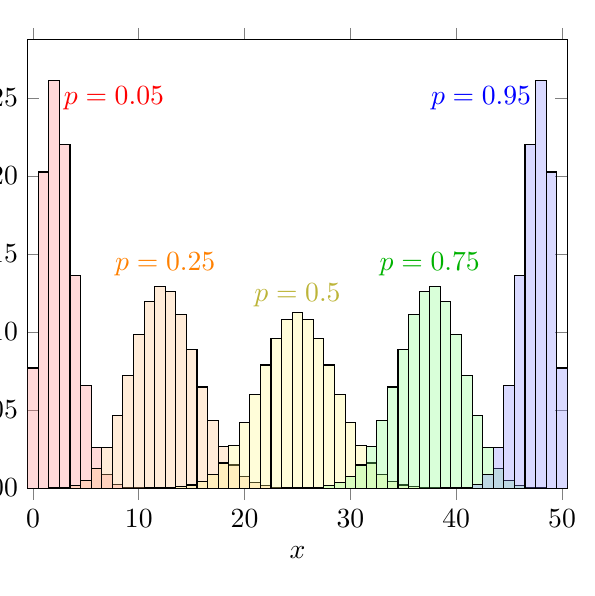
\begin{tikzpicture}[
        declare function={binom(\k,\n,\p)=\n!/(\k!*(\n-\k)!)*\p^\k*(1-\p)^(\n-\k);},
        trim axis left, trim axis right,
        ]
        \begin{axis}[
            xmin=-0.5,
            xmax=50.5,
            ymin=0,
            samples at={0,...,50},
            yticklabel style={
                /pgf/number format/fixed,
                /pgf/number format/fixed zerofill,
                /pgf/number format/precision=2
            },
            ybar=0pt,
            bar width=1,
            bar shift=0pt,
            xlabel = {$x$},
            ylabel = {$\P{X = x}$}
            ]
        \addplot[fill=red!50, fill opacity=0.3] {binom(x,50,0.05)};
        \addplot[fill=orange!50, fill opacity=0.3] {binom(x,50,0.25)};
        \addplot[fill=yellow!50, fill opacity=0.3] {binom(x,50,0.5)};
        \addplot[fill=green!50, fill opacity=0.3] {binom(x,50,0.75)};
        \addplot[fill=blue!50, fill opacity=0.3] {binom(x,50,0.95)};

        \node[red, anchor=west] at (2, 0.25) {$p = 0.05$};
        \node[orange, anchor=south] at (12.5, 0.13) {$p = 0.25$};
        \node[yellow!70!black, anchor=south] at (25, 0.11) {$p = 0.5$};
        \node[green!70!black, anchor=south] at (37.5, 0.13) {$p = 0.75$};
        \node[blue, anchor=east] at (48, 0.25) {$p = 0.95$};
        \end{axis}
    \end{tikzpicture}
    \caption{Probability distribution of $X \sim \Binom{50}{p}$ for varying values of $p$.}
\end{figure}
Notice that
\begin{itemize}
    \item when $p$ is small, the graph is right-skewed;
    \item when $p$ is large, the graph is left-skewed; and
    \item when $p = 0.5$, we get a symmetrical distribution.
\end{itemize}

A binomial distribution can only have 1 or 2 modes. If there are 2 modes, they must be consecutive integers.

\section{Poisson Distribution}

\begin{definition}
    Let $X$ be the number of occurrences of a particular event over an interval of time/space $t$. If the events
    \begin{itemize}
        \item occur independently;
        \item occur randomly and singly (the chances of multiple occurrences at precisely the same point in time/space is negligible); and
        \item occur at a constant average rate $t$ per unit time/space,
    \end{itemize}
    Then $X$ is said to follow a \vocab{Poisson distribution} with parameter $\l t$, written as $X \sim \Po{\l t}$.
\end{definition}
\begin{remark}
    Typically, we assume $t$ to be the unit interval, in which case we simply write $X \sim \Po{\l}$.
\end{remark}

Situations where a Poisson model could be used include:
\begin{itemize}
    \item the number of car accidents on a stretch of road on a random day, and
    \item the number of raisins per 10 cm$^3$ of a chocolate bar.
\end{itemize}

We can model a Poisson distribution as the sum of independent Bernoulli distributions.

\begin{proposition}
    Define $Y_i \sim \Bern{\l t / n}$ to be independent Bernoulli random variables for integers $i = 1, \dots, n$. Then, as $n \to \infty$, the sum $Y_1 + \dots + Y_n$ converges in distribution to $\Po{\l t}$.
\end{proposition}
\begin{proof}
    Consider a process in which events occur at a constant average rate $\l$ per unit time. We count the total number of events occurring over a time interval of length $t$.

    Divide the time interval down into $n$ equal subintervals of length $t/n$. For sufficiently large $n$, the probability that more than one event occurs in a subinterval is negligible. Define a Bernoulli random variable $Y_i$ for the $i$th subinterval, where
    \[Y_i = \begin{cases}1, & \text{if an event occurs in the $i$th subinterval}, \\ 0, & \ow.\end{cases}\] Since events occur independently at a constant average rate of $\l$ per unit time, the probability of success is $\l (t/n)$, so $Y_i \sim \Bern{\l t / n}$, and the total number of occurrences over the $n$ subintervals is $Y_1 + \dots + Y_n$. Taking the limit as $n \to \infty$, we get our desired result.
\end{proof}

Using Proposition~\ref{prop:drv-bin-bern}, we can use a Poisson distribution to approximate a binomial distribution.

\begin{corollary}[Poisson Limit Theorem]
    As $n \to \infty$, the binomial random variable $X \sim \Binom{n}{\l t/n}$ converges in distribution to $\Po{\l t}$.
\end{corollary}

For practical usage, this approximation is good when $n > 50$ and $p < 0.1$.

\subsection{Probability Distribution, Expectation and Variance}

\begin{proposition}[Probability Distribution of Poisson Distribution]
    Let $X \sim \Po{\l t}$. Then \[\P{X = x} = \e^{-\l t} \frac{(\l t)^x}{x!}\] for non-negative integers $x$.
\end{proposition}
The following proof uses the Poisson Limit Theorem. However, this is not the only way to derive the probability distribution. For a measure-theoretic argument, see \href{https://blog.kalculate.ai/2024/03/27/poisson-distribution/}{this blog post}. For a derivation using differential equations, see \href{https://www.pp.rhul.ac.uk/~cowan/stat/notes/PoissonNote.pdf}{this note} by Cowan.
\begin{proof}
    By the Poisson Limit Theorem, the binomial distribution $\Binom{n}{\l t / n}$ converges to $\Po{\l t}$ as $n \to \infty$. Hence, we may write \[\P{X = x} = \lim_{n \to \infty} \binom{n}{x} \bp{\frac{\l t}{n}}^x \bp{1 - \frac{\l t}{n}}^{n-x}.\] Since $n \gg x$, we have the approximations \[\binom{n}{x} = \frac{n(n-1)\dots(n-x+1)}{x!} \approx \frac{n^x}{x!} \quad \tand \quad \bp{1 - \frac{\l t}{n}}^{n-x} \approx \bp{1 - \frac{\l t}{n}}^{n} \to \e^{-\l t}.\] Thus, we obtain \[\P{X = x} = \lim_{n \to \infty} \frac{n^x}{x!} \frac{\bp{\l t}^x}{n^x} \e^{-\l t} = \e^{-\l t} \frac{\bp{\l t}^x}{x!}.\]
\end{proof}
%\begin{proof}[Proof 1 (Differential Equations).]
%    Suppose $X$ is the number of occurrences of an event over some time interval $t$. We can divide this interval into infinitely short subintervals $\D t$. For convenience, let $\P{x; t}$ be the probability that exactly $x$ events happen in the time interval $t$.
%
%    Since $\l$ is the mean rate of occurrence, we have \[\P{1; \D t} = \l \D t.\] Additionally, since $\D t$ is infinitely short, we can assume that either one event occurs, or no event occurs, i.e. \[\P{0; \D t} = 1 - \P{1; \D t} = 1 - \l \D t.\]
%
%    We now wish to find an expression for $\P{x;t}$. To do so, we first consider $\P{0;t}$. Suppose we extend the time interval $t$ by $\D t$. Since events occur independently and randomly, we must have \[\P{0;t + \D t} = \P{0; t} \P{0; \D t} = \P{0;t} \bp{1 - \l \D t}.\] We can rearrange this to get \[-\l \P{0;t} = \frac{\P{0;t + \D t} - \P{0;t}}{\D t} = \der{}{t} \P{0;t}.\] $\P{0;t}$ thus satisfies the differential equation \[\der{}{t} \P{0;t} = -\l \P{0;t},\] which has solution \[\P{0;t} = C \e^{-\l t}.\] Since no event can happen in a time interval of 0 seconds, we have \[\P{0;0} = 1 \implies C = 1.\] Thus, \[\P{0; t} = \e^{-\l t}. \tag{1}\]
%
%    We now consider $\P{x;t + \D t}$, where $x \neq 0$. If $x$ events have occurred in a time interval of $t + \D t$, one of two things must have occurred:
%    \begin{itemize}
%        \item There were $x$ events in the first $t$ seconds, but none in the last $\D t$.
%        \item There were $x-1$ events in the first $t$ seconds, and one in the last $\D t$.
%    \end{itemize}
%    We hence have
%    \begin{align*}
%        \P{x; t + \D t} &= \P{x;t}\P{0;\D t} + \P{x-1 ; t} \P{1; \D t}\\
%        &= \P{x;t} (1 - \l \D t) + \P{x-1;t} \l \D t.
%    \end{align*}
%    Rearranging, we get a differential equation involving $\P{x;t}$: \[\der{}{t} \P{x;t} + \l \P{x;t} = \l \P{x-1;t}.\] Multiplying through by the integrating factor $\e^{\l t}$, we get \[\der{}{t} \bs{\e^{\l t }\P{x;t}} = \l \e^{\l t} \P{x-1;t}. \tag{2}\]
%    
%    We now induct on (2) to get an expression for $\P{x;t}$. We claim that \[\P{x;t} = \frac{(\l t)^x}{x!} \e^{-\l t}.\] We have already shown that this holds for the $x = 0$ case. Now, substituting $x + 1$ into (2), we get \[\der{}{t} \bs{\e^{\l t }\P{x+1;t}} = \l \e^{\l t} \P{x;t} = \l \e^{\l t} \bs{\frac{(\l t)^x}{x!} \e^{-\l t}} = \frac{\l^{x+1} t^x}{x!}.\] Integrating and simplifying, we get \[\P{x+1;t} = \e^{-\l t} \int \frac{\l^{x+1} t^x}{x!} \d t = \frac{(\l t)^{x+1}}{(x+1)!} \e^{-\l t} + C \e^{-\l t}.\] Since $\P{x+1;0} = 0$, we have $C = 0$, whence \[\P{x+1;t} = \frac{(\l t)^{x+1}}{(x+1)!} \e^{-\l t}.\] This closes the induction, and we conclude that \[\P{X = x} = \P{x;t} = \frac{(\l t)^x}{x!} \e^{-\l t}.\]
%\end{proof}
%\begin{proof}%[Proof 2 (Measure Theory).]
%    Fix $t > 0$ and $\l > 0$. Suppose exactly $x$ events occur in the time interval $[0, t)$, and let their occurrence times by $0 \leq t_1 < t_2 < \dots < t_x < t$. We then define \[S_x = \bc{(t_1, \dots, t_x) \in \RR^x \mid 0 \leq t_1 < \dots < t_x < t}\] to be the set of all unordered occurrence times.
%
%    To compute the ``size'' of $S_x$, it is convenient to begin with the larger space $T = [0, t)^x$, the set of all ordered occurrence times. Since $\l$ is the mean rate of events per unit time, it is natural to introduce the measure $\m$ satisfying $\m([0, 1)) = \l$, so $\m(T) = \m([0, t)^x) = (\l t)^x$.
%    
%    Consider now the equivalence relation $\sim$ on $T$ by \[(u_1, \dots, u_x) \sim (v_1, \dots, v_x) \iff \bc{u_1, \dots, u_x} = \bc{v_1, \dots, v_x}.\] That is, two points in $T$ are equivalent if they differ only by a permutation of coordinates. Ignoring null sets where coordinates coincide, we see that each equivalence class under $\sim$ has size $x!$. Further, the quotient space $T / \sim$ may be identified (almost everywhere) with $S_x$. Thus, $S_x$ has measure \[\m(S_x) = \frac{\m(T)}{x!} = \frac{(\l t)^x}{x!}.\]
%
%    Now define the sample space \[S = \bigcup_{x = 0}^\infty S_x.\] The sets $S_x$ are disjoint, so $S$ has measure \[\m(S) = \sum_{x = 0}^\infty \m(S_x) = \sum_{x = 0}^\infty \frac{(\l t)^x}{x!} = \e^{\l t}.\]
%
%    Finally, normalizing $\m$ to a probability measure on $S$, the probability that exactly $x$ events occur in $[0, t)$ is \[\P{X = x} = \frac{\m(S_x)}{\m(S)} = \frac{(\l t)^x / x!}{\e^{\l t}} = \e^{-\l t} \frac{(\l t)^x}{x!}.\]
%\end{proof}

\begin{proposition}[Sum of Independent Poisson Random Variables is a Poisson Random Variable]
    Let $X \sim \Po{\l_1}$ and $Y \sim \Po{\l_2}$ be independent Poisson random variables. Then $X + Y \sim \Po{\l_1 + \l_2}$
\end{proposition}
\begin{proof}
    Consider the event $X + Y = n$. This can only happen if $X = m$ and $Y = n - m$ for some integer $0 \leq m \leq n$. Thus,
    \begin{align*}
        \P{X + Y = n} &= \sum_{m = 0}^n \P{X = m \tand Y = n -m}\\
        &= \sum_{m = 0}^n \P{X = m} \P{Y = n -m},
    \end{align*}
    where we used the fact that $X$ and $Y$ are independent to split the summands into products. Substituting in the probability distribution of $X$ and $Y$, we see that
    \begin{align*}
        \P{X + Y = n} &= \sum_{m = 0}^n \bs{\e^{-\l_1} \frac{\l_1^m}{m!}} \bs{\e^{-\l_2} \frac{\l_2^{n-m}}{(n-m)!}}\\
        &= \frac{\e^{-(\l_1 + \l_2)}}{n!} \sum_{m = 0}^n \frac{n!}{m! (n-m)!} \l_1^m \l_2^{n-m}\\
        &= \e^{-(\l_1 + \l_2)} \frac{(\l_1 + \l_2)^n}{n!},
    \end{align*}
    where we recognize the sum in the second line to be the binomial expansion of $(\l_1 + \l_2)^{n}$. Thus, $X + Y$ has the probability distribution of a Poisson random variable with parameter $\l_1 + \l_2$, so $X + Y \sim \Po{\l_1 + \l_2}$.
\end{proof}

This result allows us to easily approximate the sum of two binomial distributions; given $X \sim \Binom{n_1}{p_1}$ and $Y \sim \Binom{n_2}{p_2}$, we can approximate $X \sim \Po{n_1 p_1}$ and $Y \sim \Po{n_2 p_2}$ and apply the above result to get $X + Y \sim \Po{n_1 p_1 + n_2 p_2}$ (approximately).

\begin{proposition}[Expectation and Variance of Poisson Distribution]
    Let $X \sim \Po{\l t}$. Then $\E{X} = \Var{X} = \l t$.
\end{proposition}
\begin{proof}
    The binomial distribution $\Binom{n}{\l t / n}$ has mean $\l t$ and variance $n(\l t / n)(1 - \l t / n)$. Hence, by the Poisson Limit Theorem, \[\E{X} = \lim_{n \to \infty} \l t = \l t \quad \tand \quad \Var{X} = \lim_{n \to \infty} n\bp{\frac{\l t}{n}}\bp{1 - \frac{\l t}{n}} = \l t.\]
\end{proof}
%Recall that we defined $\l$ as the mean rate of occurrence per unit time. Since we measure $X$ over a time interval of length $t$, the mean number of events, $\E{X}$, is simply $\l t$. We can verify this with the following calculation:
%\begin{proof}
%    \begin{align*}
%        \E{X} &= \sum_{x = 0}^\infty  x \P{X = x}\\
%        &= \sum_{x = 1}^\infty  x \P{X = x}\\
%        &= \sum_{x = 1}^\infty  x \e^{-\l t} \frac{(\l t)^x}{x!}\\
%        &= \l t \e^{-\l t} \sum_{x = 1}^\infty \frac{(\l t)^{x-1}}{(x-1)!}\\
%        &= \l t \e^{-\l t} \sum_{x = 0}^\infty \frac{(\l t)^x}{x!}\\
%        &= \l t \e^{-\l t} \e^{\l t}\\
%        &= \l t.
%    \end{align*}
%\end{proof}
%\begin{proof}[Proof 1.]
%    Consider $\E{X^2 - X} = \E{X(X-1)}$.
%    \begin{align*}
%        \E{X(X-1)} &= \sum_{x = 0}^\infty x(x-1) \P{X = x}\\
%        &= \sum_{x = 2}^\infty x(x-1)\P{X = x}\\
%        &= (\l t)^2 \e^{-\l t} \sum_{x = 2}^\infty \frac{(\l t)^{x-2}}{(x-2)!}\\
%        &= (\l t)^2 \e^{-\l t} \e^{\l t}\\
%        &= (\l t)^2.
%    \end{align*}
%    Thus, $\E{X^2} = \E{X^2 - X} + \E{X} = (\l t)^2 + \l t$, from which it follows \[\Var{X} = \E{X^2} - \E{X}^2 = \l t.\]
%\end{proof}
%\begin{proof}%[Proof 2.]
%    Again, we begin by partitioning the time interval on which we measure $X$ into $n$ equal subdivisions. Let $Y_i$ measure the number of events that occur in the $i$th subdivision. As $n \to \infty$, each $Y_i$ approaches a point, in which case $Y_i$ follows a Bernoulli distribution with probability of success $p = \E{Y_i} = \l t / n$. Thus, \[\Var{Y_i} = p(1-p) = \frac{\l t}n \bp{1 - \frac{\l t}n}.\] Since the events occur independently, the variance of $X$ is simply the sum of the variances of $Y_i$. We thus obtain \[\Var{X} = \lim_{n \to \infty} \sum_{i = 1}^n \Var{Y_i} = \lim_{n \to \infty} \sum_{i = 0}^n \frac{\l t}n \bp{1 - \frac{\l t}n} = \lim_{n \to \infty} n\bp{\frac{\l t}{n}}\bp{1 - \frac{\l t}{n}} = \l t.\]
%\end{proof}

\subsection{Graphs of Probability Distributions}

\begin{figure}[H]\tikzsetnextfilename{417}
    \centering
    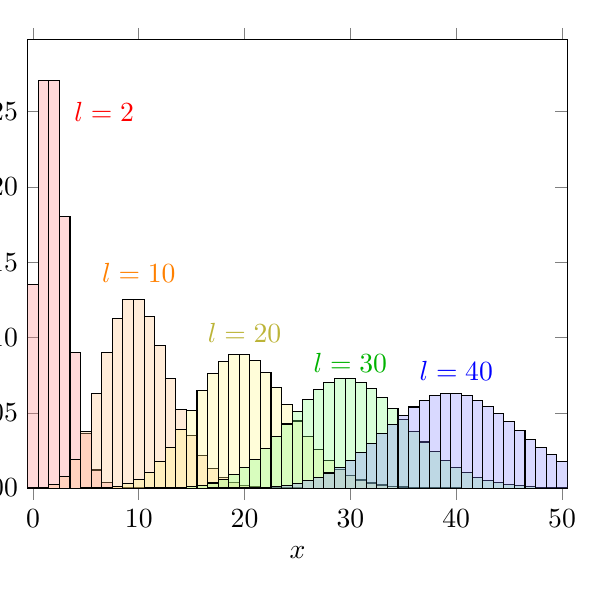
\begin{tikzpicture}[
        declare function={poisson(\k,\l)=e^(-\l) * \l^(\k) / (\k)!;},
        trim axis left, trim axis right,
        ]
        \begin{axis}[
            xmin=-0.5,
            xmax=50.5,
            ymin=0,
            samples at={0,...,50},
            yticklabel style={
                /pgf/number format/fixed,
                /pgf/number format/fixed zerofill,
                /pgf/number format/precision=2
            },
            ybar=0pt,
            bar width=1,
            bar shift=0pt,
            xlabel = {$x$},
            ylabel = {$\P{X = x}$}
            ]
        \addplot[fill=red!50, fill opacity=0.3] {poisson(x,2)};
        \addplot[fill=orange!50, fill opacity=0.3] {poisson(x,10)};
        \addplot[fill=yellow!50, fill opacity=0.3] {poisson(x,20)};
        \addplot[fill=green!50, fill opacity=0.3] {poisson(x,30)};
        \addplot[fill=blue!50, fill opacity=0.3] {poisson(x,40)};

        \node[red, anchor=west] at (3, 0.25) {$\l = 2$};
        \node[orange, anchor=south] at (10, 0.13) {$\l = 10$};
        \node[yellow!70!black, anchor=south] at (20, 0.09) {$\l = 20$};
        \node[green!70!black, anchor=south] at (30, 0.07) {$\l = 30$};
        \node[blue, anchor=south] at (40, 0.065) {$\l = 40$};
        \end{axis}
    \end{tikzpicture}
    \caption{Probability distribution of $X \sim \Po{\l}$ for varying values of $\l$.}
\end{figure}

Notice that
\begin{itemize}
    \item when $\l$ is small, the graph is right-skewed; and
    \item when $\l$ is large, we get a symmetrical distribution.
\end{itemize}

\section{Geometric Distribution}

\begin{definition}
    Suppose we keep conducting the same experiment, and let $X$ count the number of trials up to and including the first success. If
    \begin{itemize}
        \item the trials are independent;
        \item there are only two possible outcomes to each trial (``success'' and ``failure''); and
        \item the probability of ``success'', $p$, is the same for each trial,
    \end{itemize}
    then $X$ follows a \vocab{geometric distribution} with probability of success $p$, denoted $X \sim \Geo{p}$.
\end{definition}

Note that the geometric model requires the same conditions as the binomial model, with the exception that the number of trials need not be finite.

Situations where the geometric model could be applied to include:
\begin{itemize}
    \item The number of cards drawn from a pack (with replacement) before an ace is drawn.
    \item The number of times a fisherman casts a line into a river before he catches a fish.
\end{itemize}

\subsection{Probability Distribution, Expectation and Variance}

\begin{proposition}[Probability Distribution of Geometric Distribution]
    Let $X \sim \Geo{p}$. Then $\P{X = x} = (1-p)^{x-1} p$ for positive integers $x$.
\end{proposition}
\begin{proof}
    By definition, the event $X = x$ can only occur if the previous $x - 1$ trials are failures (which occur with probability $1-p$), and the $x$th trial is a success (which occurs with probability $p$). Thus, by the Multiplication Principle, $\P{X = x} = \bp{1 - p}^{x-1} p$.
\end{proof}

The geometric distribution has the following useful property:
\begin{proposition}
    Let $X \sim \Geo{p}$. Then $\P{X > x} = (1-p)^x$.
\end{proposition}
\begin{proof}%[Proof 1.]
    The event $X > x$ is equivalent to the event that the first $x$ trials were all failures. Thus, $\P{X = x} = (1-p)^x$.
\end{proof}
%\begin{proof}[Proof 2 (Probability Distribution).]
%    We have \[\P{X > x} = \sum_{k = x + 1}^\infty \P{X = k} = \sum_{k = x+1}^\infty (1-p)^{k-1} p.\] This is simply an infinite geometric series with common ratio $1-p$ and first term $(1-p)^x p$. Thus, \[\P{X > x} = \frac{(1-p)^x p}{1 - (1-p)} = (1-p)^x.\]
%\end{proof}

This actually implies a much stronger property about the geometric distribution:

\begin{definition}
    A random variable $X$ is said to be \vocab{memoryless} if, for all non-negative $s$ and $t$, we have $\P{X > s + t}{X > t} = \P{X > s}$.
\end{definition}

\begin{proposition}[Geometric Distribution is Memoryless]
    Let $X \sim \Geo{p}$. Then $X$ is memoryless.
\end{proposition}
\begin{proof}
    We have
    \begin{align*}
        \P{X > s + t}{X > t} &= \frac{\P{X > s + t \tand X > t}}{\P{X > t}}\\
        &= \frac{\P{X > s + t}}{\P{X > t}}\\
        &= \frac{(1-p)^{s+t}}{(1-p)^t}\\
        &= (1-p)^s\\
        &= \P{X > s}.
    \end{align*}
\end{proof}

This result aligns with our intuition; since each trial is independent, the ``waiting time'' for a success does not depend on how much ``time'' has already passed.

\begin{proposition}[Expectation and Variance of Geometric Distribution]
    Let $X \sim \Geo{p}$. Then \[\E{X} = \frac1p \quad \tand \Var{X} = \frac{1-p}{p^2}.\]
\end{proposition}
Intuitively, since each trial has probability of success $p$, we expect $p$ successes for every 1 trial. This is equivalent to 1 success every $1/p$ trials, so $\E{X} = 1/p$. Of course, we can prove this fact more rigorously:
%\begin{proof}[Proof 2 (Probability Distribution).]
%    \[\E{X} = \sum_{k = 1}^\infty k \P{X = k} = p \sum_{k = 1}^\infty k (1-p)^{k-1}.\] Recall that the Maclaurin series of $(1 - x)^{-2}$ is \[\frac1{(1-x)^{2}} = \sum_{k = 1}^\infty k x^{k-1}.\] Substituting $1-p$ for $x$, we get \[\E{X} = \frac{p}{p^2} = \frac{1}{p}.\]
%\end{proof}
\begin{proof}
    Let $A$ and $B$ be the event that the first trial is a success and a failure respectively.
    \begin{itemize}
        \item If $A$ occurs (with probability $p$), the process stops, and $\E{X}{A} = 1$.
        \item If $B$ occurs (with probability $1-p$), by the memoryless property, the process effectively ``restarts''. Hence, the expected number of trials in this case becomes $\E{X}{B} = \E{1 + X} = 1 + \E{X}$.
    \end{itemize}

    By the law of total expectation, we obtain the equation \[\E{X} = \P{A} \E{X}{A} + \P{B} \E{B}{A} = (p)(1) + (1-p)\E{1 + X}.\] Solving for $\E{X}$, we get $\E{X} = 1/p$.

    Again, by the law of total expectation,
    \begin{align*}
        \E{X^2} &= \P{A} \E{X^2}{A} + \P{B} \E{X^2}{B}\\
        &= (p)(1)^2 + (1-p)\E{(1 + X)^2}\\
        &= p + (1-p)\bs{1 + \frac2p + \E{X^2}}
    \end{align*}
    Solving for $\E{X^2}$, we have \[\E{X^2} = \frac{2-p}{p^2},\] so \[\Var{X} = \E{X^2} - \E{X}^2 = \frac{1-p}{p^2}.\]
\end{proof}

%\begin{proposition}[Variance of Geometric Distribution]
%    Let $X \sim \Geo{p}$. Then \[\Var{X} = \frac{1-p}{p^2}.\]
%\end{proposition}
%\begin{proof}[Proof 1 (Probability Distribution).]
%    Recall that \[\sum_{k = 1}^\infty x^k = \frac{1}{1 - x}.\] Differentiating this twice with respect to $x$, we get \[\sum_{k = 1}^\infty k(k-1) x^{k-2} = \frac{2}{(1-x)^3} \implies \sum_{k = 1}^\infty \bp{k^2 - k} x^{k-1} = \frac{2x}{(1-x)^3}. \tag{1}\]
%
%    Now consider $\E{X^2} - \E{X}$: \[\E{X^2} - \E{X}= \sum_{k = 1}^\infty \bp{k^2 - k} \P{X = k} = p \sum_{k = 1}^\infty \bp{k^2 - k} (1-p)^{k-1}.\] Using (1) with $x = 1-p$, \[\E{X^2} - \E{X} = p \bs{\frac{2(1-p)}{p^3}} = \frac{2 - 2p}{p^2}.\] Thus, \[\E{X^2} = \frac{2 - 2p}{p^2} + \frac1p = \frac{2-p}{p^2} \implies \Var{X} = \E{X^2} - \E{X}^2 = \frac{1-p}{p^2}.\]
%\end{proof}

\subsection{Graphs of Probability Distribution}

\begin{figure}[H]\tikzsetnextfilename{423}
    \centering
    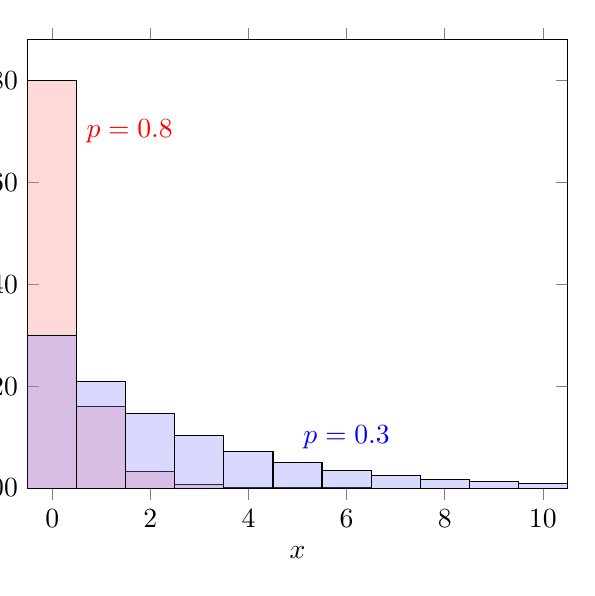
\begin{tikzpicture}[
        declare function={geom(\k,\p)=(1-\p)^\k * \p;},
        trim axis left, trim axis right,
        ]
        \begin{axis}[
            xmin=-0.5,
            xmax=10.5,
            ymin=0,
            samples at={0,...,10},
            yticklabel style={
                /pgf/number format/fixed,
                /pgf/number format/fixed zerofill,
                /pgf/number format/precision=2
            },
            ybar=0pt,
            bar width=1,
            bar shift=0pt,
            xlabel = {$x$},
            ylabel = {$\P{X = x}$}
            ]
        \addplot[fill=red!50, fill opacity=0.3] {geom(x,0.8)};
        \addplot[fill=blue!50, fill opacity=0.3] {geom(x,0.3)};

        \node[red, anchor=west] at (0.5, 0.7) {$p = 0.8$};
        \node[blue] at (6, 0.1) {$p = 0.3$};
        \end{axis}
    \end{tikzpicture}
    \caption{Probability distribution of $X \sim \Geo{p}$ for varying values of $p$.}
\end{figure}

All geometric distributions demonstrate extreme right-skewness.